\documentclass{article}
\usepackage{graphicx} % Required for inserting images
\usepackage{amsmath}
\usepackage{amssymb}
\usepackage{floatrow}
\usepackage{changepage}
\usepackage{float}

\title{Elliptic Filter Design Report}
\author{Name: Geetesh Kini, Roll no: 210070041, Filter no: 104, Group No: 15,\\ Reviewed by Group member: Chanakya Varude, Roll no: 210070092}
\date{February 2023}

\begin{document}

\maketitle

\tableofcontents
\clearpage

\section{Filter Details (Bandpass)}

\subsection{Un-normalized Discrete Time Filter Specifications}

Filter number = 104\\
Since filter number $>$ 80, m = 104 - 80 = 24\\
q(m) = greatest integer strictly less than 0.1*m = 2\\
r(m) = m - 10*q(m) = 4\\
$B_L$(m) = 10 + 5*q(m) + 13*r(m) = 10 + 5*2 + 13*4 = 72KHz \\
$B_H$(m) = $B_L$(m) + 75 = 147KHz\\

\vspace{1.5em}
\noindent

This filter is given to be a Bandpass Filter with passband from BL(m) kHz to BH(m) kHz.
Therefore the specifications are:
\begin{itemize}
    \item Passband : \textbf{72 - 147 KHz}
    \item  Transition band : \textbf{5KHz} on either side of stopband
    \item Stopband : \textbf{0 - 67} and \textbf{152 - 300 KHz} (As \textbf{sampling rate} is \textbf{600KHz})

    \item  Tolerance : \textbf{0.15} in \textbf{magnitude} for both passband and stopband
    \item  Nature : Both Passband and Stopband are \textbf{equiripple}
\end{itemize}

\subsection{Normalized Digital Filter Specifications}
Sampling rate = 600KHz\\
In the normalized frequency axis, sampling rate corresponds to 2$\pi$\\
Therefore, any frequency can be normalized as follows :
\begin{equation*}
    \omega = \frac{\Omega*2\pi}{\Omega_s}
\end{equation*}
where $\Omega_s$ is the Sampling Rate.\\

\vspace{1em}
\noindent
For the normalized discrete filter specifications, the nature and tolerances being the dependent variables remain the same while the passband and stopband frequencies change as per the above transformations. 
\begin{itemize}
    \item Passband : (\textbf{0.24 -  0.49}) {$\pi$}
    \item  Transition band : \textbf{0.017} $\pi$ on either side of stopband
    \item Stopband : (\textbf{0 - 0.223}) {$\pi$} and (\textbf{0.507 - 1}) {$\pi$}
    \item  Tolerance : \textbf{0.15} in \textbf{magnitude} for both passband and stopband
    \item Passband nature: \textbf{Equiripple}
    \item Stopband nature: \textbf{Equiripple}
\end{itemize}


\subsection{Band-pass analog Filter Specifications using Bilinear
Transformation}
To convert to analog domain, we use the following transformation :
\begin{equation*}
    \Omega = \tan (\frac{w}{2})
\end{equation*}
Applying the transformation at Band Edges we get :
\begin{table}[H]
		% Center the table
		\begin{center}
		\begin{tabular}{|c|c|}
			% To create a horizontal line, type \hline
			\hline
			% To end a column type &
			% For a linebreak type \\
			$\omega$ & $\Omega$\\
			
			\hline
                0 & 0\\
                \hline
                0.24 $\pi$ & 0.396 \\
                \hline
                0.49 $\pi$ & 0.969\\
                \hline
                0.223 $\pi$ & 0.365\\
                \hline
                0.507 $\pi$ & 1.022\\
                \hline
                $\pi$ & $\infty$\\
                \hline
            
		\end{tabular}
		\end{center}
\end{table}

Hence, the specifications for corresponding bandpass analog filter are:
\begin{itemize}
    \item Passband : (\textbf{0.396 -  0.969})
    \item  Transition band : \textbf{0.365 to 0.396} and \textbf{0.969 to 1.022}
    \item Stopband : (\textbf{0 - 0.365}) and (\textbf{1.022 - $\infty$})
    \item  Tolerance : \textbf{0.15} in \textbf{magnitude} for both passband and stopband
    \item Passband nature: \textbf{Equiripple}
    \item Stopband nature: \textbf{Equiripple}
\end{itemize}

\subsection{Low pass analog Filter Specifications using Frequency
Transformation}

We need to transform the bandpass filter to a low pass filter. Hence, we can use the bandpass transformation:
\vspace{-5mm}
\begin{center}
    \begin{equation*}
        \Omega_L = \frac{\Omega^2-\Omega_0^2}{B\Omega}
    \end{equation*}
\end{center}

Where $\Omega_0$ and B can be determined by:
We want $\Omega_{P1}$ to map to -1 and $\Omega_{P2}$ to map to +1.\\
Using this, we get:
\begin{center}
    \begin{equation*}
        \Omega_0 = \sqrt{\Omega_{P1}\Omega_{P2}} = \sqrt{0.396 \times 0.969} = 0.61945
    \end{equation*}
    \begin{equation*}
        B = \Omega_{P2} - \Omega_{P1} = 0.969 - 0.396 = 0.573
    \end{equation*}
\end{center}

\begin{table}[H]
		% Center the table
		\begin{center}
		\begin{tabular}{|c|c|}
			% To create a horizontal line, type \hline
			\hline
			% To end a column type &
			% For a linebreak type \\
			$\Omega$ & $\Omega_L$\\
			
			\hline
                $0^+$ & - $\infty$\\
                \hline
                0.365($\Omega_{S1}$) & -1.198$\Omega_{L_{S1}}$)\\
                \hline
                0.396($\Omega_{P1}$) & -1($\Omega_{L_{P1}}$)\\
                \hline
                0.61945($\Omega_0$) & 0\\
                \hline
                0.969($\Omega_{P2}$) & +1($\Omega_{L_{P2}}$) \\
                \hline
                1.022($\Omega_{S2}$) & 1.128$\Omega_{L_{S2}}$)\\
                \hline
                $\infty$ & $\infty$\\
                \hline
            
		\end{tabular}
		\end{center}
\end{table}

\subsection{Low pass Analog filter specifications}

\begin{itemize}
    \item Passband Edge : 1 ($\Omega_{L_{P}}$)
    \item Stopband Edge : min(-$\Omega_{L_{S1}}$, $\Omega_{L_{S2}}$) = min(1.198, 1.128) = 1.128 ($\Omega_{L_{S}}$)
    \item  Tolerance : \textbf{0.15} in \textbf{magnitude} for both passband and stopband
    \item Passband nature: \textbf{Equiripple}
    \item Stopband nature: \textbf{Equiripple}
\end{itemize}

\subsection{Analog Lowpass Transfer Function}

The analog filter has both passband and stopband Equiripple, hence, we need a \textbf{Elliptic} filter.\\

The Low pass transfer function for it is given by:
\begin{center}
    \begin{equation*}
        H_{LPF}(s_L)H_{LPF}(-s_L) = \frac{1}{1+\epsilon^2U^2_N(\frac{s_L}{j})}
    \end{equation*}
\end{center}

Where $U_N(\Omega_L) = cd(N \times u \times K_1,k_1)$ where u is such that $\Omega_L = cd(u \times K(k),k)$, and cd is one of the general Jacobi elliptic functions. Here, K(k) is given by the equation:

\begin{center}
         K(k) = \(\int_{0}^{1} \frac{1}{(1-t^2)(1-kt^2)} \,dt\)
\end{center}

Where the parameters are given by:

\begin{center}
    \begin{equation*}
        \epsilon = \sqrt{\frac{2\delta_1-\delta_1^2}{1-2\delta_1+\delta_1^2}}
    \end{equation*}
\end{center}

\begin{center}
   $
        k_1 = \frac{\epsilon}{\sqrt{\frac{1}{\delta_2^2}-1}}$,       
       $ k_1'=\sqrt{1-k_1^2}
    $
\end{center}

\begin{center}
    $k=\frac{1}{\Omega_{s_L}}$,   $k'=\sqrt{1-k^2}$
\end{center}

\begin{center}
    $N = ceil(\frac{K(k)K'(k_1)}{K'(k)K(k_1)})$
\end{center}

Substituting values, we get, $\epsilon$ = 0.6197, $k_1$ = 0.940, k = $\frac{1}{1.128}$ = 0.8865\\
Using MATLAB, we can compute K(k), and other integrals, and we get the value of N to be 4. Hence for this value of N, the modified values of k and $\Omega_{s_L}$ we get are k = 0.9595 and $\Omega_{s_L}$ = 1.0422\\

Now, N can be represented as 2l+r, where r $\in$ \{0,1\}\\, and it turns out that $U_N$ can be written as:

\begin{equation}
    U_N(\Omega) = (\Omega)^r\Pi_{i=1}^l\left[\left(\frac{\Omega^2-\zeta_i^2}{1-\Omega^2k^2\zeta_i^2}\right)\cdot\left(\frac{1-k^2\zeta_i^2}{1-\zeta_i^2}\right)\right]
\end{equation}

where

\begin{equation*}
    u_i = \frac{2i-1}{N}\text{ ; where } i \in {1,2,...,l}
\end{equation*}
\begin{equation*}
    \zeta_i = cd(u_i\cdot K(k),k) = \textit{cde}(u_i,k)
\end{equation*}

Hence the zeroes of $U_N$ are given by:
\begin{equation}
    z_i = \frac{j}{k\zeta_i}\text{ ; where } i \in {1,2,...,l}
\end{equation}
Remaining zeroes are $z_i^*$ i.e. conjugates of $z_i$\\
Here, as N=4, we have l=2, r=0.

Hence, the zeroes are:\\
$z_1$=j/(0.9595*0.9796)=1.0639j\\
$z_2$=j/(0.9595*0.5891)=1.769j\\
$z_1^*$= -1.0639j \\
$z_2^*$= -1.7690j\\

And the poles are given by:\\
There are 2l+r i.e. N poles to $|H(j\Omega)|$\\
Let v $\in \mathbb{R}$ be a solution to $sn(jv\cdot N\cdot K(k),k)$ = j/$\epsilon_p$, therefore
\begin{equation}
    v = \frac{-j}{N\cdot K(k)}sn^{-1}(\frac{j}{\epsilon_p},k_1) = \frac{-j}{N}asne(\frac{j}{\epsilon_p},k_1)
\end{equation}
Poles are given by:
\begin{equation}
    p_i = jcd((u_i-jv)K(k),k) = jcde(u_i-jv,k)\text{ ,where } i\in {1,2,...,l}
\end{equation}
\begin{equation}
    p_0 = jcd((1-jv)K(k),k) = jcde(1-jv,k)
\end{equation}
$p_0$ is the pole on negative real axis which occurs only when r=1.

Hence in this case, using MATLAB, we get that the poles are:\\
$p_1$= -0.0310 + 0.9995i\\
$p_2$= -0.3536 + 0.7071i\\
$p_1^*$= -0.0310 - 0.9995i \\
$p_2^*$= -0.3536 - 0.7071i\\

\begin{equation}
    H_{analog\_LP}(s) = \frac{0.15s^4 + 0.6392s^2 + 0.5313}{1s^4 + 0.7691s^3 + 1.6689s^2 + 0.7459s + 0.6251}
\end{equation}

Here, the leading coefficient on the numerator is obtained by scaling the numerator such that ratio of constant terms of the numerator and denominator equals the value of $H_{analog\_LP}(0)$. Here, $H_{analog\_LP}(0)$ turns out to be 0.85 by substituting the values of $\epsilon$ and $U_N(0)$, and also, 0.5313/0.6251 = 0.85

\subsection{Analog Bandpass Transfer Function}

The transformation is given by:
\vspace{-5mm}
\begin{center}
    \begin{equation*}
        s_L = \frac{\Omega_0^2+s^2}{Bs}
    \end{equation*}
\end{center}

Substituting $\Omega_0$ and B, we get:

\begin{equation*}
    H_{analog\_BP}(s) =\frac{(0.1500s^8 + 0.4402s^6 + 0.3509s^4 + 0.0648s^2 + 0.0033)}{1s^8 + 0.4408s^7 + 2.0829s^6 + 0.6478s^5 + 1.3714s^4 + 0.2486s^3 + 0.3066s^2 + 0.0249s + 0.0217}
\end{equation*}

\subsection{Discrete Time Filter Transfer Function}

Now, performing the bilinear transform, i.e. $s = \frac{1-z^{-1}}{1+z^{-1}}$ gives us:

\begin{center}
$H_{discrete\_BS}(z) = \frac{0.1642z^8 - 0.4354z^7 + 0.7986z^6 - 1.0930z^5 + 1.2667z^4 - 1.0930z^3 + 0.7986z^2 - 0.4354z + 0.1642}{1z^8 - 2.9661z^7 +  6.0876z^6 - 8.3174z^5 + 9.0890z^4 - 7.2019z^3 + 4.5490z^2 - 1.8939z + 0.5567}$    
\end{center}

Hence, this, is the final discrete time transfer function of our Elliptic bandpass filter.
\clearpage

\subsection{Matlab Plots}

\begin{figure}[h!]

\centering
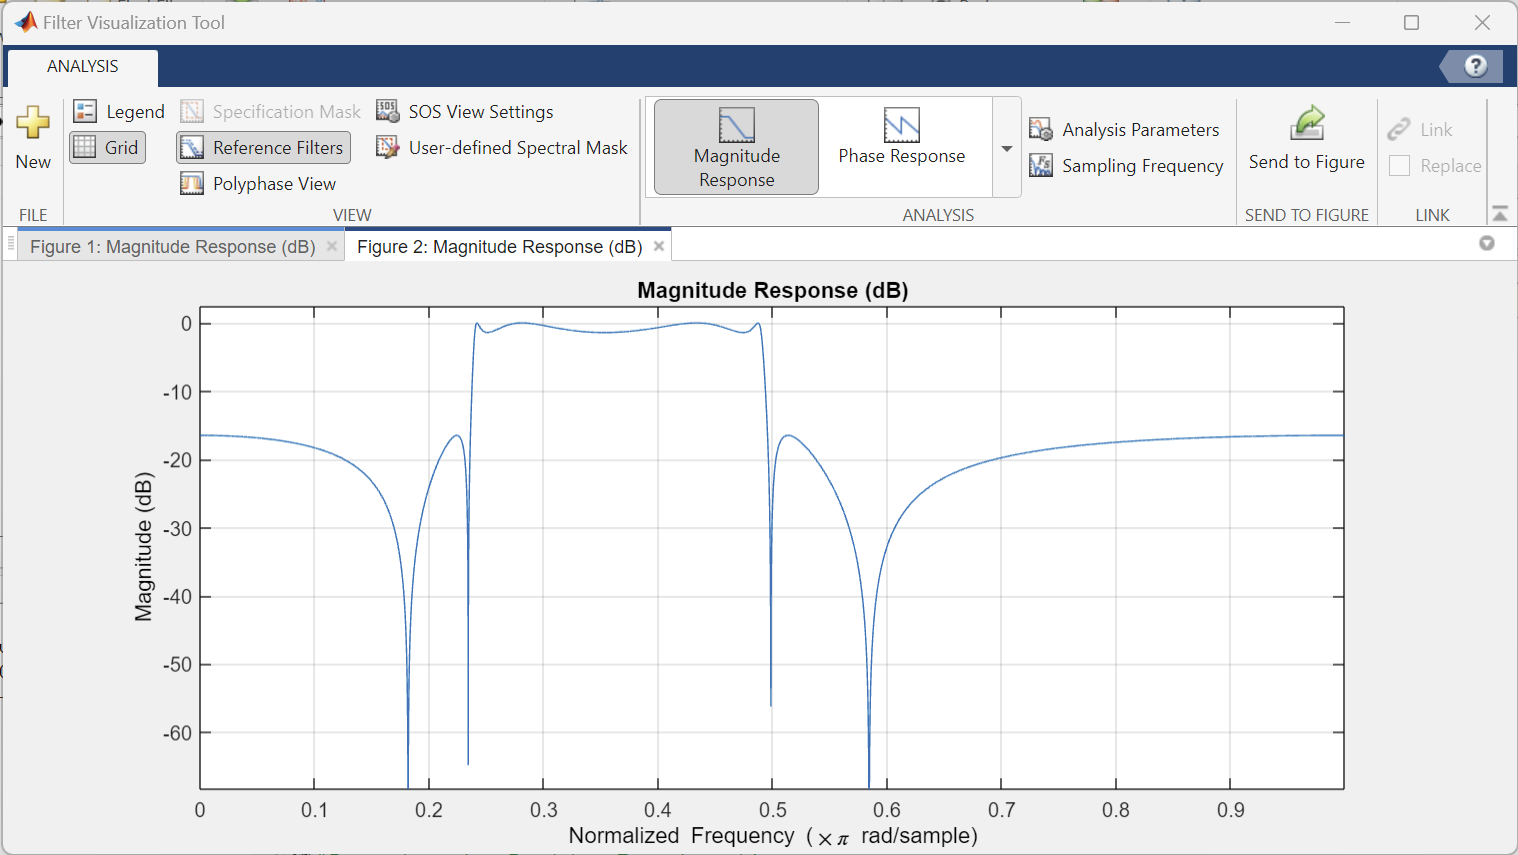
\includegraphics[scale = 0.5]{Elliptic_Magnitude_BandPass.png}
\caption{Magnitude Plot in dB}
\end{figure}

\begin{figure}[h!]

\centering
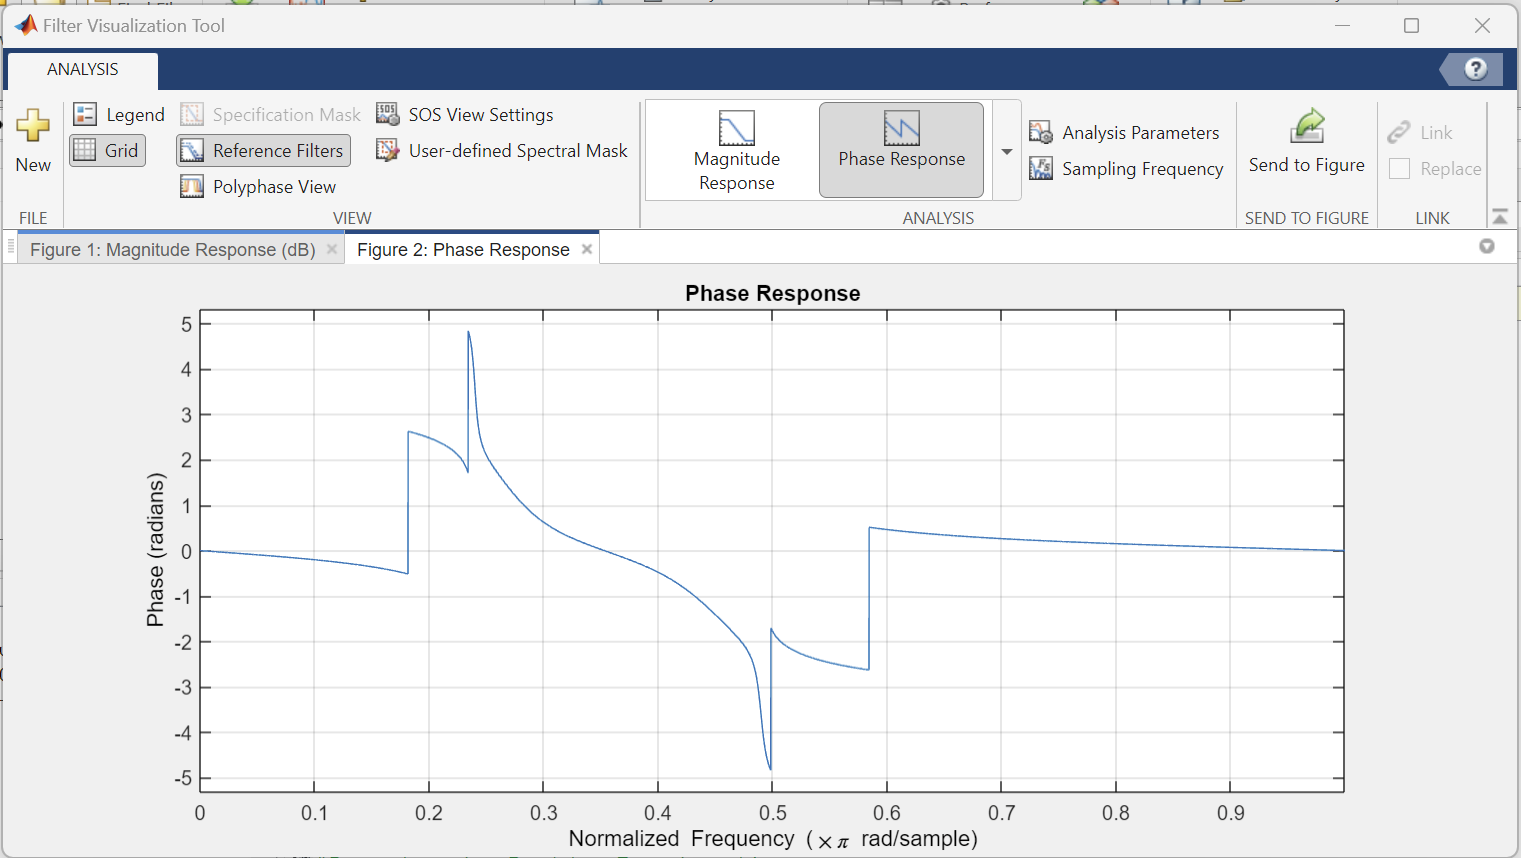
\includegraphics[scale = 0.5]{Elliptic_Phase_BandPass.png}
\caption{Phase Response}
\end{figure}

We can see that the Phase Response is \textbf{not} linear.

\begin{figure}[h!]

\centering
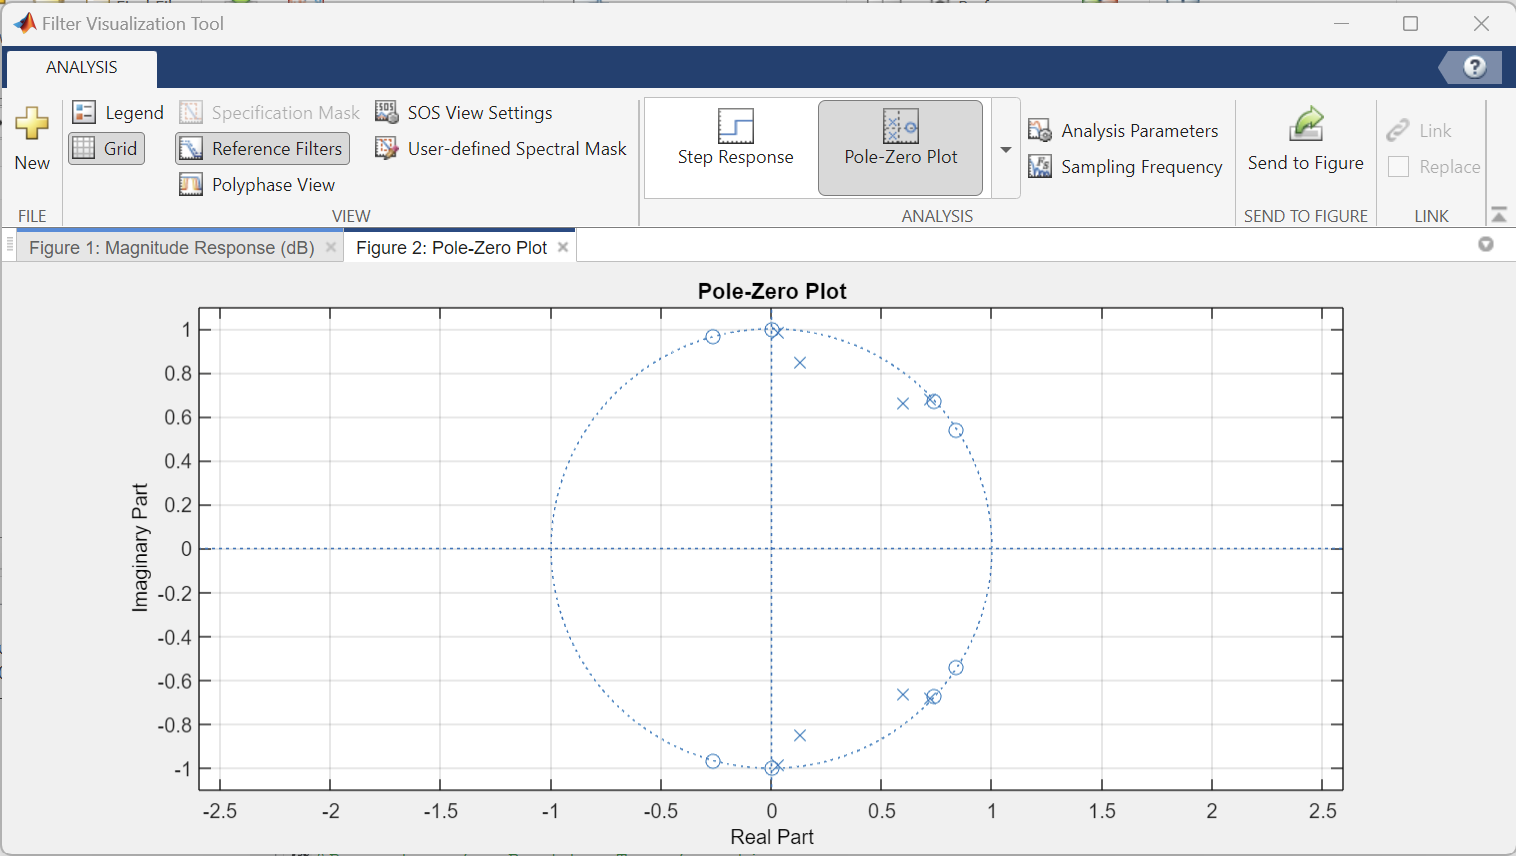
\includegraphics[scale = 0.5]{Elliptic_Pole_Bandpass.png}
\caption{Poles and Zeroes}
\end{figure}

We can see that all the poles lie inside the unit circle and hence, the system is stable.

\begin{figure}[h!]

\centering
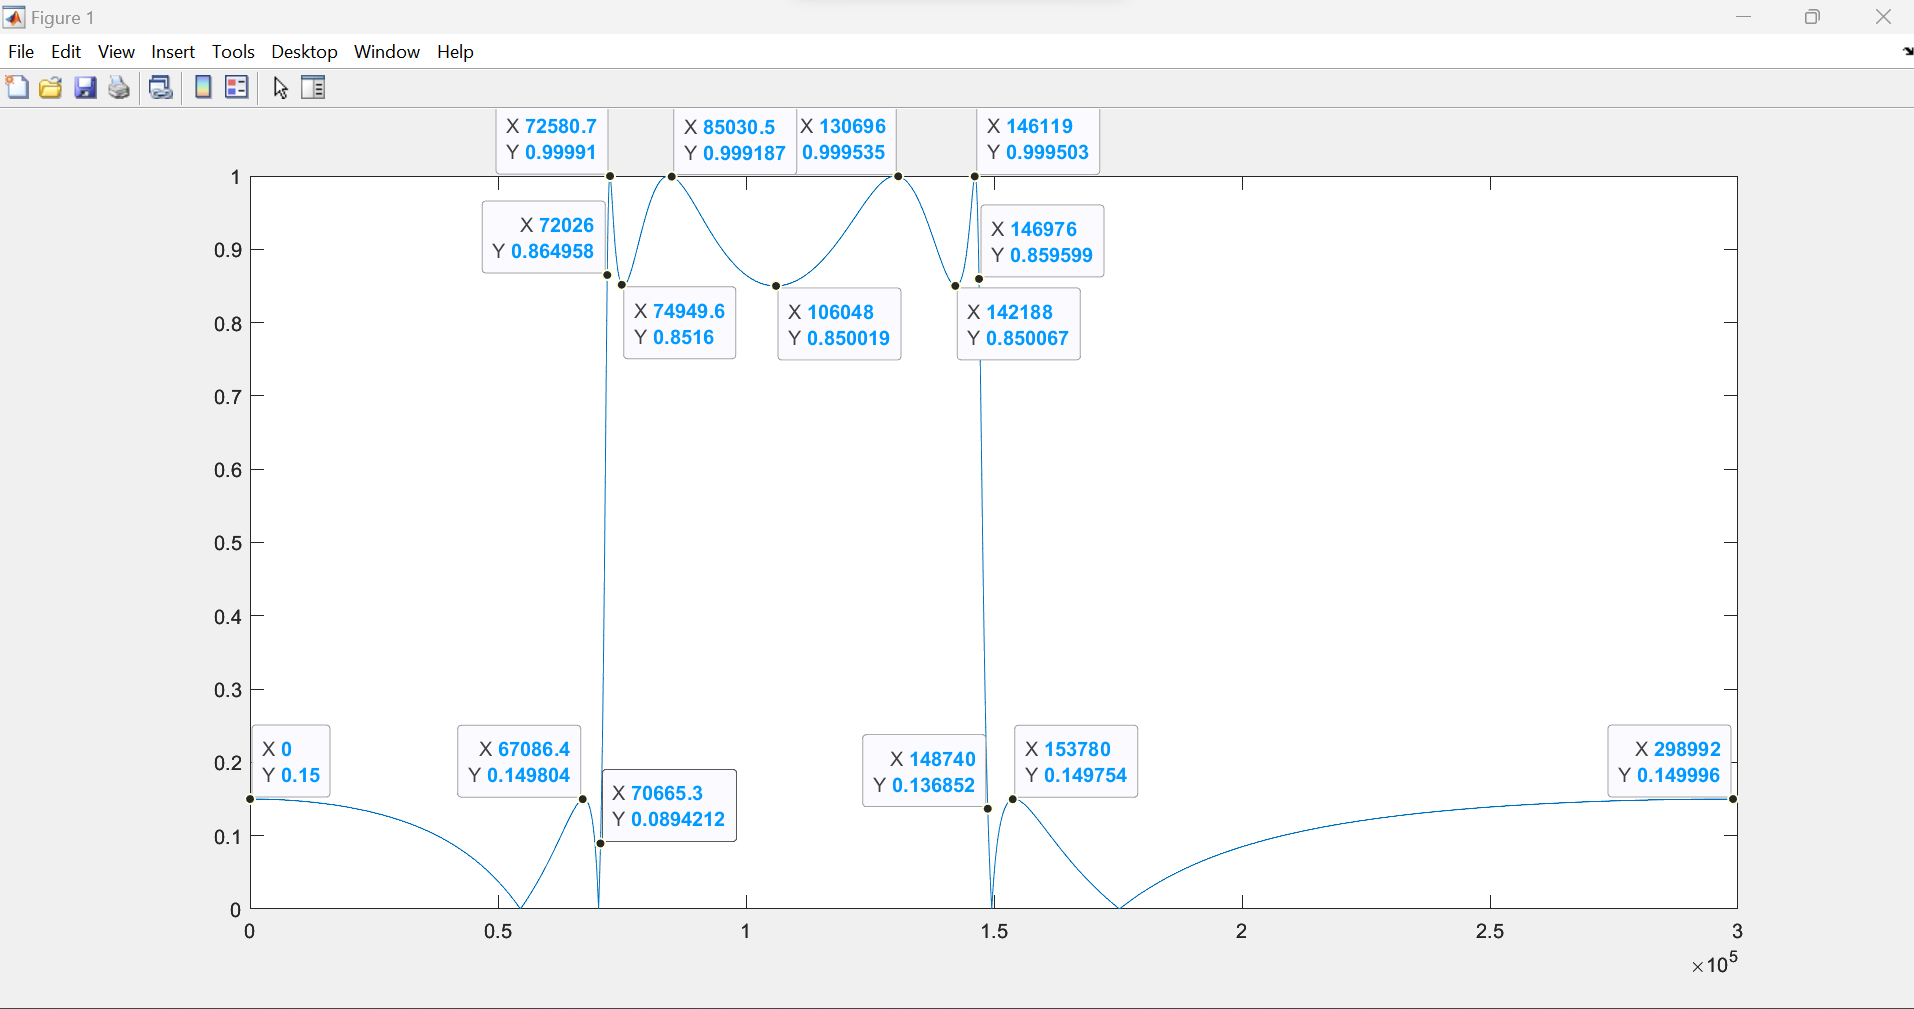
\includegraphics[scale = 0.4]{Elliptic_freq_BandPass.png}
\caption{Magnitude Plot}
\end{figure}

From the above figure, we can see that all the specifications are satisfied.

\subsection{Observations on elliptical filter design and comparisons with Chebyschev, FIR methods}

I had also designed Bandpass filters with the same specifications except nature of Passband and Stopband with Chebyschev and FIR filters. So I noticed the following things about the 3 filters:

\begin{itemize}
    \item For the same PassBand and StopBand frequencies, the order, i.e. the amount of resources we need is the least for elliptic filters, and highest for FIR filters.
    \item Also, in the Magnitude plot, I observed that FIR filters don't have much Ripple, whereas in Elliptic and Chebyschev, the ripples are such that it just satisfies the specifications. Also, in Elliptic and Chebyschev filters, the gain is never more than 1, but in FIR filters, the gain also lies between 1 and 1 + (PassBand tolerance).
    \item We can’t control the tolerances of passband and stopband independently in FIR filters. In both Chebyschev and Elliptic filters, we can do that.
    \item The Phase Response is linear (as we preferably want) in FIR filter, whereas it's non linear in both Elliptic and Chebyschev Filters.
\end{itemize}

So, each type of filter has its own advantage, we can choose the one we want according to our needs.

\clearpage

\section{Filter Details (Bandstop)}
\subsection{Un-normalized Discrete Time Filter Specifications}

Filter number = 104\\
Since filter number $>$ 80, m = 104 - 80 = 24\\
q(m) = greatest integer strictly less than 0.1*m = 2\\
r(m) = m - 10*q(m) = 4\\
$B_L$(m) = 20 + 3*q(m) + 11*r(m) = 20 + 3*2 + 11*4 = 70KHz \\
$B_H$(m) = $B_L$(m) + 40 = 110KHz\\

\vspace{1.5em}
\noindent

This filter is given to be a Bandstop Filter with stopband from BL(m) kHz to BH(m) kHz.
Therefore the specifications are:
\begin{itemize}
    \item Stopband : \textbf{70 - 110 KHz}
    \item  Transition band : \textbf{5KHz} on either side of stopband
    \item Passband : \textbf{0 - 65} and \textbf{115 - 212.5 KHz} (As \textbf{sampling rate} is \textbf{425KHz})

    \item  Tolerance : \textbf{0.15} in \textbf{magnitude} for both passband and stopband
    \item  Nature : Both passband and stopband are \textbf{Equiripple}
\end{itemize}


\subsection{Normalized Digital Filter Specifications}
Sampling rate = 425KHz\\
In the normalized frequency axis, sampling rate corresponds to 2$\pi$\\
Therefore, any frequency can be normalized as follows :
\begin{equation*}
    \omega = \frac{\Omega*2\pi}{\Omega_s}
\end{equation*}
where $\Omega_s$ is the Sampling Rate.\\

\vspace{1em}
\noindent
For the normalized discrete filter specifications, the nature and tolerances being the dependent variables remain the same while the passband and stopband frequencies change as per the above transformations. 
\begin{itemize}
    \item Stopband : (\textbf{0.329 -  0.518}) {$\pi$}
    \item  Transition band : \textbf{0.024} $\pi$ on either side of stopband
    \item Passband : (\textbf{0 - 0.306}) {$\pi$} and (\textbf{0.541 - 1}) {$\pi$}
    \item  Tolerance : \textbf{0.15} in \textbf{magnitude} for both passband and stopband
    \item Passband nature: \textbf{Equiripple}
    \item Stopband nature: \textbf{Equiripple}
\end{itemize}

\subsection{Band-stop analog Filter Specifications using Bilinear
Transformation}
To convert to analog domain, we use the following transformation :
\begin{equation*}
    \Omega = \tan (\frac{w}{2})
\end{equation*}
Applying the transformation at Band Edges we get :
\begin{table}[H]
		% Center the table
		\begin{center}
		\begin{tabular}{|c|c|}
			% To create a horizontal line, type \hline
			\hline
			% To end a column type &
			% For a linebreak type \\
			$\omega$ & $\Omega$\\
			
			\hline
                0 & 0\\
                \hline
                0.329 $\pi$ & 0.568 \\
                \hline
                0.518 $\pi$ & 1.058\\
                \hline
                0.306 $\pi$ & 0.521\\
                \hline
                0.541 $\pi$ & 1.137\\
                \hline
                $\pi$ & $\infty$\\
                \hline
            
		\end{tabular}
		\end{center}
\end{table}

Hence, the specifications for corresponding bandstop analog filter are:
\begin{itemize}
    \item Stopband : (\textbf{0.568 -  1.058})
    \item  Transition band : \textbf{0.521 to 0.568} and \textbf{1.058 to 1.137}
    \item Passband : (\textbf{0 - 0.521}) and (\textbf{1.137 - $\infty$})
    \item  Tolerance : \textbf{0.15} in \textbf{magnitude} for both passband and stopband
    \item Passband nature: \textbf{Equiripple}
    \item Stopband nature: \textbf{Equiripple}
\end{itemize}

\subsection{Low pass analog Filter Specifications using Frequency
Transformation}

We need to transform the bandstop filter to a low pass filter. Hence, we can use the bandstop transformation:
\vspace{-5mm}
\begin{center}
    \begin{equation*}
        \Omega_L = \frac{B\Omega}{\Omega_0^2-\Omega^2}
    \end{equation*}
\end{center}

Where $\Omega_0$ and B can be determined by:
We want $\Omega_{P1}$ to map to +1 and $\Omega_{P2}$ to map to -1.\\
Using this, we get:
\begin{center}
    \begin{equation*}
        \Omega_0 = \sqrt{\Omega_{P1}\Omega_{P2}} = \sqrt{0.521 \times 1.137} = 0.76966
    \end{equation*}
    \begin{equation*}
        B = \Omega_{P2} - \Omega_{P1} = 1.137 - 0.521 = 0.616
    \end{equation*}
\end{center}

\begin{table}[H]
		% Center the table
		\begin{center}
		\begin{tabular}{|c|c|}
			% To create a horizontal line, type \hline
			\hline
			% To end a column type &
			% For a linebreak type \\
			$\Omega$ & $\Omega_L$\\
			
			\hline
                $0^+$ & $0^+$\\
                \hline
                0.521($\Omega_{P1}$) & +1($\Omega_{L_{P1}}$) \\
                \hline
                0.568($\Omega_{S1}$) & 1.297$\Omega_{L_{S1}}$)\\
                \hline
                0.76966($\Omega_0^-$) & $\infty$\\
                \hline
                0.76966($\Omega_0^+$) & - $\infty$\\
                \hline
                1.058($\Omega_{S2}$) & -1.236$\Omega_{L_{S2}}$)\\
                \hline
                1.137($\Omega_{P2}$) & -1($\Omega_{L_{P2}}$)\\
                \hline
                $\infty$ & $0^-$\\
                \hline
            
		\end{tabular}
		\end{center}
\end{table}

\subsection{Low pass Analog filter specifications}

\begin{itemize}
    \item Passband Edge : 1 ($\Omega_{L_{P}}$)
    \item Stopband Edge : min($\Omega_{L_{S1}}$, -$\Omega_{L_{S2}}$) = min(1.297, 1.236) = 1.236 ($\Omega_{L_{S}}$)
    \item  Tolerance : \textbf{0.15} in \textbf{magnitude} for both passband and stopband
    \item Passband nature: \textbf{Equiripple}
    \item Stopband nature: \textbf{Equiripple}
\end{itemize}

\subsection{Analog Lowpass Transfer Function}

The analog filter has both passband and stopband Equiripple, hence, we need a \textbf{Elliptic} filter.\\

The Low pass transfer function for it is given by:
\begin{center}
    \begin{equation*}
        H_{LPF}(s_L)H_{LPF}(-s_L) = \frac{1}{1+\epsilon^2U^2_N(\frac{s_L}{j})}
    \end{equation*}
\end{center}

Where $U_N(\Omega_L) = cd(N \times u \times K_1,k_1)$ where u is such that $\Omega_L = cd(u \times K(k),k)$, and cd is one of the general Jacobi elliptic functions. Here, K(k) is given by the equation:

\begin{center}
         K(k) = \(\int_{0}^{1} \frac{1}{(1-t^2)(1-kt^2)} \,dt\)
\end{center}

Where the parameters are given by:

\begin{center}
    \begin{equation*}
        \epsilon = \sqrt{\frac{2\delta_1-\delta_1^2}{1-2\delta_1+\delta_1^2}}
    \end{equation*}
\end{center}

\begin{center}
   $
        k_1 = \frac{\epsilon}{\sqrt{\frac{1}{\delta_2^2}-1}}$,       
       $ k_1'=\sqrt{1-k_1^2}
    $
\end{center}

\begin{center}
    $k=\frac{1}{\Omega_{s_L}}$,   $k'=\sqrt{1-k^2}$
\end{center}

\begin{center}
    $N = ceil(\frac{K(k)K'(k_1)}{K'(k)K(k_1)})$
\end{center}

Substituting values, we get, $\epsilon$ = 0.6197, $k_1$ = 0.940, k = $\frac{1}{1.236}$ = 0.8091\\
Using MATLAB, we can compute K(k), and other integrals, and we get the value of N to be 3. Hence for this value of N, the modified values of k and $\Omega_{s_L}$ we get are k = 0.8571 and $\Omega_{s_L}$ = 1.1667\\

Now, N can be represented as 2l+r, where r $\in$ \{0,1\}\\, and it turns out that $U_N$ can be written as:

\begin{equation}
    U_N(\Omega) = (\Omega)^r\Pi_{i=1}^l\left[\left(\frac{\Omega^2-\zeta_i^2}{1-\Omega^2k^2\zeta_i^2}\right)\cdot\left(\frac{1-k^2\zeta_i^2}{1-\zeta_i^2}\right)\right]
\end{equation}

where

\begin{equation*}
    u_i = \frac{2i-1}{N}\text{ ; where } i \in {1,2,...,l}
\end{equation*}
\begin{equation*}
    \zeta_i = cd(u_i\cdot K(k),k) = \textit{cde}(u_i,k)
\end{equation*}

Hence the zeroes of $U_N$ are given by:
\begin{equation}
    z_i = \frac{j}{k\zeta_i}\text{ ; where } i \in {1,2,...,l}
\end{equation}
Remaining zeroes are $z_i^*$ i.e. conjugates of $z_i$\\
Here, as N=3, we have l=1, r=1.

Hence, the zeroes are:\\
$z_1$=j/(0.8571*0.9256)=1.1261j\\
$z_1^*$= -1.1261j \\

And the poles are given by:\\
There are 2l+r i.e. N poles to $|H(j\Omega)|$\\
Let v $\in \mathbb{R}$ be a solution to $sn(jv\cdot N\cdot K(k),k)$ = j/$\epsilon_p$, therefore
\begin{equation}
    v = \frac{-j}{N\cdot K(k)}sn^{-1}(\frac{j}{\epsilon_p},k_1) = \frac{-j}{N}asne(\frac{j}{\epsilon_p},k_1)
\end{equation}
Poles are given by:
\begin{equation}
    p_i = jcd((u_i-jv)K(k),k) = jcde(u_i-jv,k)\text{ ,where } i\in {1,2,...,l}
\end{equation}
\begin{equation}
    p_0 = jcd((1-jv)K(k),k) = jcde(1-jv,k)
\end{equation}
$p_0$ is the pole on negative real axis which occurs only when r=1.

Hence in this case, using MATLAB, we get that the poles are:\\
$p_0$= -0.6232\\
$p_1$= -0.1153 + 0.9936i\\
$p_1^*$= -0.1153 - 0.9936i \\


\begin{equation}
    H_{analog\_LP}(s) = \frac{0.3925s^2 + 0.6235}{1s^3 + 0.8539s^2 + 1.1443s + 0.6235}
\end{equation}

Here, the leading coefficient on the numerator is obtained by scaling the numerator such that ratio of constant terms of the numerator and denominator equals the value of $H_{analog\_LP}(0)$. Here, $H_{analog\_LP}(0)$ turns out to be 1 by substituting the values of $\epsilon$ and $U_N(0)$, and also, we can see that the constant terms of the num and den are equal.

\subsection{Analog Bandpass Transfer Function}

The transformation is given by:
\vspace{-5mm}
\begin{center}
    \begin{equation*}
        s_L = \frac{Bs}{\Omega_0^2+s^2}
    \end{equation*}
\end{center}

Substituting $\Omega_0$ and B, we get:

\begin{equation*}
    H_{analog\_BP}(s) =\frac{(1s^6 + 2.0201s^4 + 1.1988s^2 + 0.2090)}{1s^6 + 1.1329s^5 + 2.3020s^4 + 1.7218s^3 + 1.3661s^2 + 0.3989s + 0.2090}
\end{equation*}

\subsection{Discrete Time Filter Transfer Function}

Now, performing the bilinear transform, i.e. $s = \frac{1-z^{-1}}{1+z^{-1}}$ gives us:

\begin{center}
$H_{discrete\_BS}(z) = \frac{0.5446z^6 - 0.7858z^5 + 1.8345z^4 - 1.5417z^3 + 1.8345z^2 - 0.7858z + 0.5446}{1z^6 - 1.1751z^5 + 2.0860z^4 - 1.4853z^3 + 1.4725z^2 - 0.4529z + 0.1997}$    
\end{center}

Hence, this, is the final discrete time transfer function of our Elliptic bandpass filter.
\clearpage

\subsection{Matlab Plots}

\begin{figure}[h!]

\centering
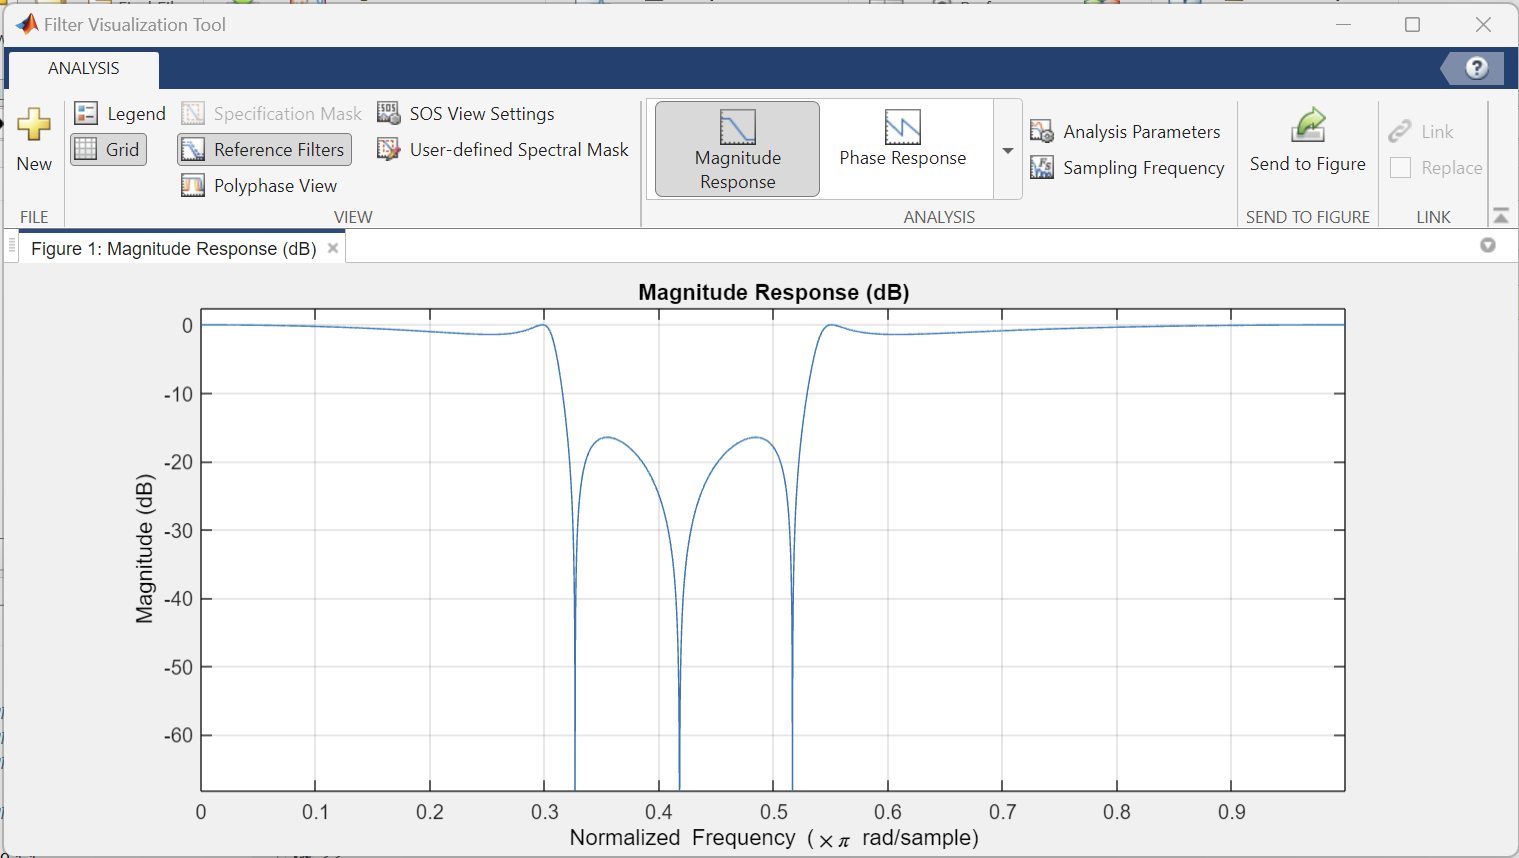
\includegraphics[scale = 0.5]{Elliptic_Magnitude_BandStop.png}
\caption{Magnitude Plot in dB}
\end{figure}

\begin{figure}[h!]

\centering
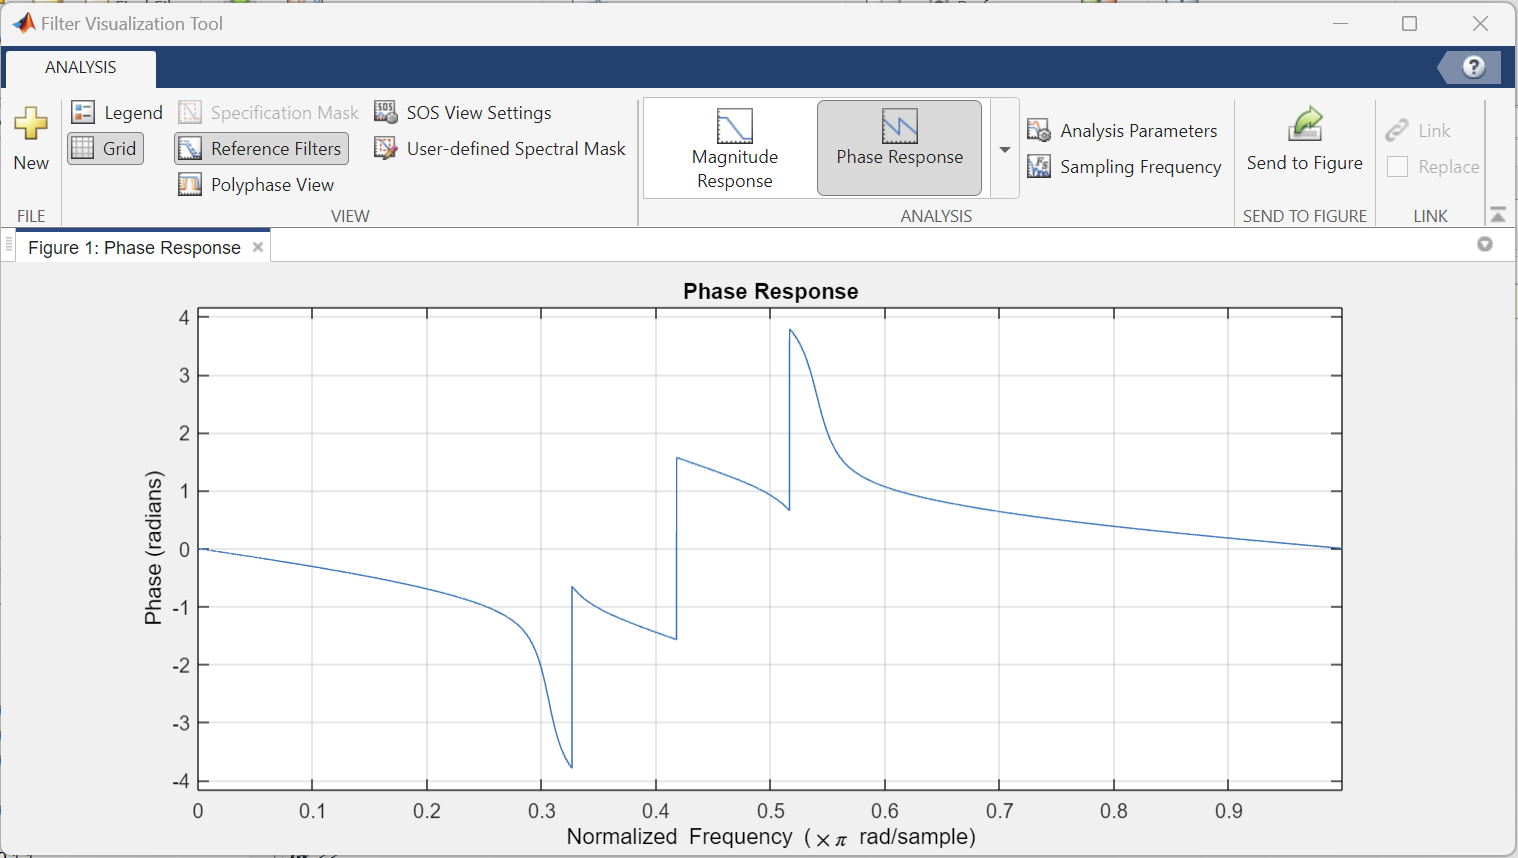
\includegraphics[scale = 0.5]{Elliptic_Phase_BandStop.png}
\caption{Phase Response}
\end{figure}

We can see that the Phase Response is \textbf{not} linear.

\begin{figure}[h!]

\centering
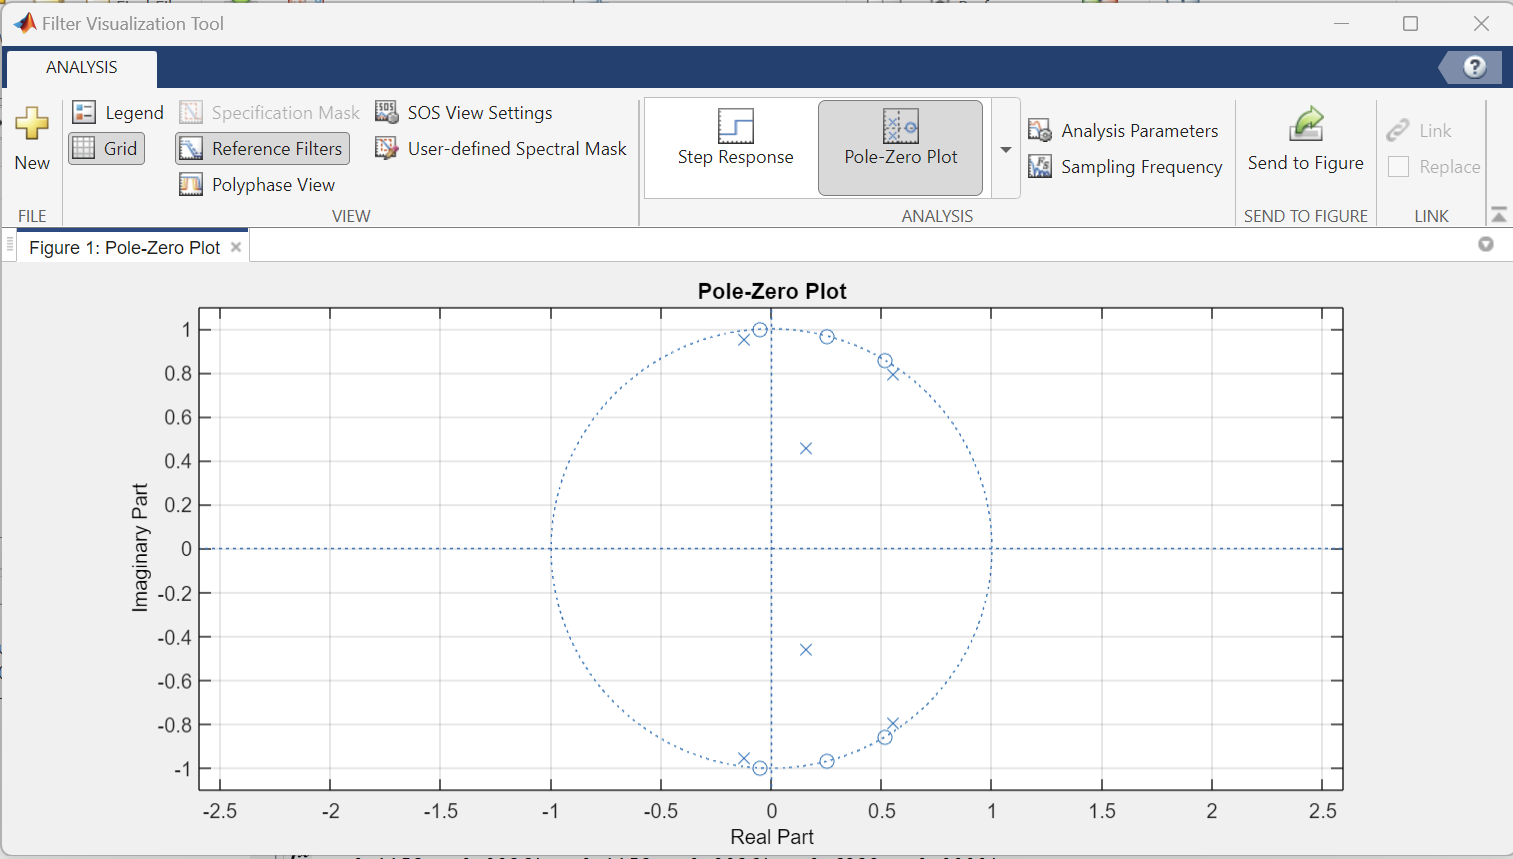
\includegraphics[scale = 0.5]{Elliptic_Pole_Bandstop.png}
\caption{Poles and Zeroes}
\end{figure}

We can see that all the poles lie inside the unit circle and hence, the system is stable.

\begin{figure}[h!]

\centering
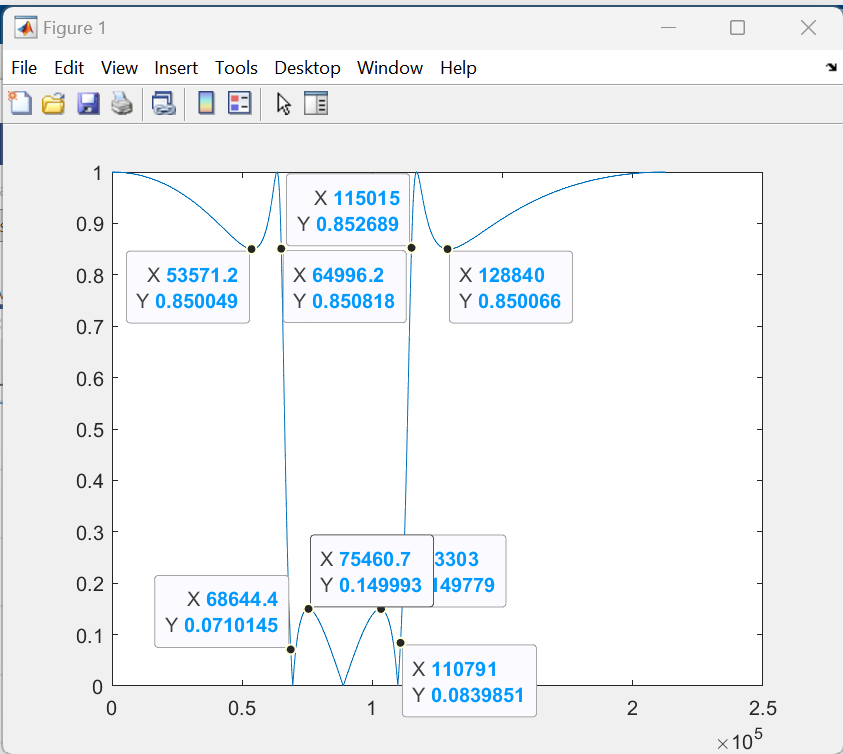
\includegraphics[scale = 0.58]{Elliptic_freq_BandStop.png}
\caption{Magnitude Plot}
\end{figure}

From the above figure, we can see that all the specifications are satisfied.

\subsection{Observations on elliptical filter design and comparisons with Butterworth, FIR methods}

I had also designed Bandstop filters with the same specifications except nature of Passband and Stopband with Butterworth and FIR filters. So I noticed the following things about the 3 filters:

\begin{itemize}
    \item For the same PassBand and StopBand frequencies, the order, i.e. the amount of resources we need is the least for elliptic filters, and highest for FIR filters.
    \item Also, in the Magnitude plot, I observed that FIR filters don't have much Ripple, whereas in Elliptic, the ripples are such that it just satisfies the specifications and Butterworth doesn't have any ripples at all. Also, in Elliptic and Butterworth filters, the gain is never more than 1, but in FIR filters, the gain also lies between 1 and 1 + (PassBand tolerance).
    \item We can’t control the tolerances of passband and stopband independently in FIR filters. In both Butterworth and Elliptic filters, we can do that.
    \item The Phase Response is linear (as we preferably want) in FIR filter, whereas it's non linear in both Elliptic and Butterworth Filters.
\end{itemize}

So, each type of filter has its own advantage, we can choose the one we want according to our needs.

\section{Peer Review of Assignment}

I have reviewed the report of my peer:

\begin{center}
    Annirudh K P\\
    (Roll no: 210070009, Filter number: 96)
\end{center}
and certify it to be correct.

\end{document}

\end{document}
